\documentclass[a4paper,12pt]{article}
%%% Default imports
\usepackage{listings} % Code listings
\usepackage{graphicx} % Images
\usepackage{booktabs} % Better tables
\usepackage{makecell}
\usepackage{enumitem} % Lists
\usepackage{dsfont}
\usepackage{geometry} % Page geometry
\usepackage[utf8]{inputenc} % Encoding
\usepackage[T2A]{fontenc} % Font
\usepackage[english, russian]{babel} % Multi-language support
\usepackage{titling} % Better titles
\usepackage{textcomp} % Old-style numbers? Check difference
\usepackage{mathtext} % Russian text in math expressions? Check difference
\usepackage{amsmath, amsfonts, amssymb, amsthm, mathtools} % Mathematics
\usepackage{bm} % Bold math symbols
\usepackage{icomma} % Better comma in numbers within math mode
\usepackage{xifthen} % Better if-expressions
\usepackage{transparent} % Transparent colors
\usepackage{caption}    % }
\usepackage{subcaption} % } Captioning figures
\usepackage[table,xcdraw]{xcolor} % Colors
\usepackage{textpos} % Absolute positioning
\usepackage{upgreek} % Cool greek letters

\usepackage{fancyvrb}
\usepackage{fvextra}
\usepackage{chngcntr}

%%% Page geometry
\setlength\parindent{0pt} % No indentation between paragraphs
\setlist{noitemsep} % No spacing between list items

\usepackage{float}
\usepackage{multirow}

\geometry{
    paper=a4paper,
    top=2.5cm,
    bottom=3cm,
    left=2.5cm,
    right=2.5cm,
    headheight=0.75cm,
    footskip=1.5cm,
    headsep=0.75cm,
}

%%% Numeration
\newcommand{\RNumb}[1]{\uppercase\expandafter{\romannumeral #1\relax}}
\newcommand{\thesec}{\arabic{section}}
\renewcommand\thesection{\arabic{section}}
\renewcommand\thesubsection{\thesection.\arabic{subsection}}
\renewcommand\thesubsubsection{\RNumb{\arabic{subsubsection}}}
\renewcommand{\sectionmark}[1]{\markright{\thesection\ #1}}
\renewcommand{\bf}{\textbf}
\renewcommand{\it}{\textit}
\def\hash{\texttt{\#}}
\def\cpp{\C\texttt{++}}

\counterwithin{figure}{section}
\counterwithin{table}{section}
\renewenvironment{titlepage}{\thispagestyle{empty}} % Include titlepage into page numeration

%%% Headers and footers
\usepackage{setspace}
\usepackage{fancyhdr}
\usepackage{lastpage}


%%% Graphics
% Custom colors
\definecolor{myblue}{RGB}{72, 184, 178}
\definecolor{myblue1}{RGB}{0, 109, 167}
\definecolor{commentgreen}{RGB}{2,112,10}
\definecolor{mauve}{rgb}{0.58,0,0.82}
\definecolor{amethyst}{RGB}{153, 102, 203}

\usepackage{pgfplots} % Plots
\usepackage{tikz}
\usetikzlibrary{3d,perspective,decorations.text}
\usetikzlibrary{animations}
\usetikzlibrary{positioning}
\usetikzlibrary{matrix}
\usepackage{tikz-cd}
\usetikzlibrary{cd}
\usetikzlibrary{karnaugh}
\pgfplotsset{width=6cm,compat=newest}
\usepackage{color}

\usepackage[framemethod=TikZ]{mdframed}
\newcommand{\definebox}[2]{\newcounter{#1}\newenvironment{#1}[1][]{\stepcounter{#1}\mdfsetup{frametitle={\tikz[baseline=(current bounding box.east),outer sep=0pt]\node[anchor=east,rectangle,fill=white]{\strut \MakeUppercase#1~\csname the#1\endcsname\ifstrempty{##1}{}{:~##1}};}}\mdfsetup{innertopmargin=1pt,linecolor=#2,linewidth=3pt,topline=true,frametitleaboveskip=\dimexpr-\ht\strutbox\relax,}\begin{mdframed}[]\relax}{\end{mdframed}}}
\definebox{definition}{black!90}
\definebox{theorem}{myblue1!90}
\definebox{demonstration}{amethyst!90}

\newcounter{Theorem}
\def\themytheorem{\thesection.\arabic{Theorem}}
\usepackage[most]{tcolorbox}
\tcbuselibrary{theorems}
\newtcbtheorem{Theorem}{Theorem}
{colframe=myblue!90,coltitle=black,colback=white,fonttitle=\bfseries}{Th}

%%% Code listings
\usepackage{matlab-prettifier}

\lstdefinestyle{cpp} {
    language=C++,
    frame=tb,
    tabsize=4,
    showstringspaces=false,
    numbers=left,
    captionpos=b,
    columns=flexible,
    upquote=true,
    commentstyle=\color{commentgreen},
    keywordstyle=\color{blue},
    stringstyle=\color{commentgreen},
    basicstyle=\small\ttfamily,
    emph={int,char,double,float,unsigned,void,bool,size\_t},
    emphstyle={\color{blue}},
    escapechar=\&,
    classoffset=1,
    otherkeywords={>,<,.,;,-,!,=,~},
    morekeywords={>,<,.,;,-,!,=,~},
    keywordstyle=\color{black},
    classoffset=0,
}
\lstdefinestyle{def} {
    frame=tb,
    tabsize=4,
    showstringspaces=false,
    numbers=left,
    captionpos=b,
    columns=flexible,
    upquote=true,
    commentstyle=\color{black},
    keywordstyle=\color{black},
    stringstyle=\color{black},
    basicstyle=\small\ttfamily,
    emph={int,char,double,float,unsigned,void,bool,size\_t},
    emphstyle={\color{black}},
    escapechar=\&,
    classoffset=1,
    otherkeywords={>,<,.,;,-,!,=,~},
    morekeywords={>,<,.,;,-,!,=,~},
    keywordstyle=\color{black},
    classoffset=0,
}
\lstdefinelanguage[RISC-V]{Assembler}
{
    alsoletter={.}, % allow dots in keywords
    alsodigit={0x}, % hex numbers are numbers too!
    morekeywords=[1]{ % instructions
    lb, lh, lw, lbu, lhu,
    sb, sh, sw,
    sll, slli, srl, srli, sra, srai,
    add, addi, sub, lui, auipc,
    xor, xori, or, ori, and, andi,
    slt, slti, sltu, sltiu,
    beq, bne, blt, bge, bltu, bgeu,
    j, jr, jal, jalr, ret,
    scall, break, nop
},
    morekeywords=[2]{ % sections of our code and other directives
    .align, .ascii, .asciiz, .byte, .data, .double, .extern,
    .float, .globl, .half, .kdata, .ktext, .set, .space, .text, .word
},
    morekeywords=[3]{ % registers
    zero, ra, sp, gp, tp, s0, fp,
    t0, t1, t2, t3, t4, t5, t6,
    s1, s2, s3, s4, s5, s6, s7, s8, s9, s10, s11,
    a0, a1, a2, a3, a4, a5, a6, a7,
    ft0, ft1, ft2, ft3, ft4, ft5, ft6, ft7,
    fs0, fs1, fs2, fs3, fs4, fs5, fs6, fs7, fs8, fs9, fs10, fs11,
    fa0, fa1, fa2, fa3, fa4, fa5, fa6, fa7
},
    morecomment=[l]{;},   % mark ; as line comment start
    morecomment=[l]{\#},  % as well as # (even though it is unconventional)
    morestring=[b]",      % mark " as string start/end
    morestring=[b]'       % also mark ' as string start/end
}
\lstdefinestyle{riscv} {
    basicstyle=\small\ttfamily,                    % very small code
    breaklines=true,                              % break long lines
    commentstyle=\itshape\color{green!50!black},  % comments are green
    keywordstyle=[1]\color{blue!80!black},        % instructions are blue
    keywordstyle=[2]\color{orange!80!black},      % sections/other directives are orange
    keywordstyle=[3]\color{red!50!black},         % registers are red
    stringstyle=\color{mauve},                    % strings are from the telekom
    identifierstyle=\color{teal},                 % user declared addresses are teal
    frame=l,                                      % black line on the left side of code
    captionpos=b,
    language=[RISC-V]Assembler,                   % all code is RISC-V
    tabsize=4,                                    % indent tabs with 4 spaces
    showstringspaces=false                        % do not replace spaces with weird underlines
}

%%% Other
\usepackage[normalem]{ulem} % }
\useunder{\uline}{\ul}{}    % } Underline text
\usepackage[colorlinks,urlcolor=blue,filecolor=blue,citecolor=blue,linkcolor = blue,unicode=true]{hyperref}
\usepackage{titlesec}
\titlelabel{\thetitle.\quad}
\usepackage{secdot}
\sectiondot{subsection}
\usepackage{kvmap} % Karnaugh-maps for logic functions
\usepackage{}
\newcommand{\projectname}[3]{
    \begin{center}
        \Large
        \textbf{#1}\\[10pt]
        \textbf{#2}\\[10pt]
        \normalsize
        #3
        \rule{\linewidth}{0.4pt}
    \end{center}
}

\newcommand{\hfconfiguration}[3]{
    \pagestyle{fancy}
    \fancyhead[LE,RO]{}
    \fancyhead[LO,RE]{#1}
    \renewcommand{\footrulewidth}{0.4pt}
    \fancyfoot[C]{\thepage/\pageref*{LastPage}}
    \fancyfoot[LO,RE]{#2}
    \fancyfoot[LE,RO]{#3}
}

\newcommand{\filename}[2]{
    \pagebreak
    \titleformat{\section}
    [display]
    {\bfseries\Large}
    {}
    {0ex}
    {
        \vspace{-4.5ex}
        % \rule{\textwidth}{1pt}
        #1 \centering
    % \vspace{1ex}
    }
    [
        \normalfont\large
        #2
        \rule{\textwidth}{0.4pt}
        \normalsize
    ]
}

\newcommand{\project}[6]{
    \projectname{#1}{#2}{#3}
    \pagestyle{empty}
    \tableofcontents
    \newpage
    \hfconfiguration{#4}{#5}{#6}
}
%%% Final touch
\usepackage{subfiles}


\begin{document}
    \begin{titlepage}
    \begin{center}
        \large Санкт-Петербургский политехнический университет Петра Великого\\
        \large Институт компьютерных наук и технологий \\
        \large Кафедра компьютерных систем и программных технологий\\[6cm]


        \huge Отчет по лабораторной работе №3\\[0.5cm]
        \large по дисциплине <<Схемотехника операционных устройств>>\\[0.1cm]
        \large\textbf{Триггеры}\\[5cm]
    \end{center}


    \begin{flushright}
        \begin{minipage}{0.25\textwidth}
            \begin{flushleft}

                \large\textbf{Работу выполнил:}\\
                \large Ильин В.П.\\
                \large {Группа:} 35300901/10005\\

                \large \textbf{Преподаватель:}\\
                \large Киселев И.О.

            \end{flushleft}
        \end{minipage}
    \end{flushright}

    \vfill

    \begin{center}
        \large Санкт-Петербург\\
        \large \the\year
    \end{center}
\end{titlepage}

\vfill
\newpage

    \tableofcontents

    \section{Цели работы}
    \begin{itemize}
        \item Закрепление знаний и получение практических навыков синтеза комбинационных схем в заданном
        элементном базисе.
        \item Получение навыков ввода проекта в графическом редакторе пакета QП, тестирования и отладки проекта и
        исследования на модели рисков сбоев.
        \item Получение навыков отладки цифровых устройств данного класса на физической модели: конфигурирование ПЛИС и
        экспериментальная проверка работы комбинационной схемы при использовании лабораторной платы miniDiLab.
    \end{itemize}

    \section{Задача}
	В соответствии с вариантом, составить таблицу истинности для логической функции 5 переменных. Минимизировать функцию при помощи карт
	Карно. Синтезировать комбинационную схему и исследовать ее при помощи САПР Quartus Prime. Реализовать полученную
	комбинационную схему на физической модели.
	
	Исходная функция задана таблично:
	\begin{table}[H]
		\centering
		\begin{tabular}{|c|c|}
		\hline Для значений $y = 1$ & Для значений $y = \textit{н}$ \\
		\hline $1, 6-10, 13, 15, 20-25, 28, 31$ & $3, 4, 12, 17, 26$ \\
		\hline
		\end{tabular}
	\end{table}
    \section{Ход работы}
    \subsection{Получение таблицы истинности}
    Для построения таблицы истинности необходимо перебрать все возможные
    наборы значений аргументов и указать данное значение $y_{\text{исх}}$ для каждого набора.
    Столбец $y_{\text{теор}}$ соответствует выбранным значениям для наборов <<н>>, столбец
    $y_{\text{эксп}}$ -- значениям, полученным в процессе тестирования комбинационной схемы,
    $y_{\text{физ}}$ -- значениям, полученным в процессе тестирования физической схемы.
    \begin{table}[H]
		\centering
		\begin{tabular}{|c|c|c|c|c|c|c|c|c|c|}
		\hline
		№ & $x_1$ & $x_2$ & $x_3$ & $x_4$ & $x_5$ & $y_{\text{исх}}$ & $y_{\text{теор}}$ & $y_{\text{эксп}}$ & $y_{\text{физ}}$ \\
		\hline 
		0 & 0 & 0 & 0 & 0 & 0 & 0 & 0 & 0 & 0 \\
		\hline 
		1 & 0 & 0 & 0 & 0 & 1 & 1 & 1 & 1 & 1 \\
		\hline 
		2 & 0 & 0 & 0 & 1 & 0 & 0 & 0 & 0 & 0 \\
		\hline 
		3 & 0 & 0 & 0 & 1 & 1 & н & 0 & 0 & 0 \\
		\hline 
		4 & 0 & 0 & 1 & 0 & 0 & н & 0 & 0 & 0 \\
		\hline 
		5 & 0 & 0 & 1 & 0 & 1 & 0 & 0 & 0 & 0 \\
		\hline 
		6 & 0 & 0 & 1 & 1 & 0 & 1 & 1 & 1 & 1 \\
		\hline 
		7 & 0 & 0 & 1 & 1 & 1 & 1 & 1 & 1 & 1 \\
		\hline 
		8 & 0 & 1 & 0 & 0 & 0 & 1 & 1 & 1 & 1 \\
		\hline 
		9 & 0 & 1 & 0 & 0 & 1 & 1 & 1 & 1 & 1 \\
		\hline 
		10 & 0 & 1 & 0 & 1 & 0 & 1 & 1 & 1 & 1 \\
		\hline 
		11 & 0 & 1 & 0 & 1 & 1 & 0 & 0 & 0 & 0 \\
		\hline 
		12 & 0 & 1 & 1 & 0 & 0 & н & 1 & 1 & 1 \\
		\hline 
		13 & 0 & 1 & 1 & 0 & 1 & 1 & 1 & 1 & 1 \\
		\hline 
		14 & 0 & 1 & 1 & 1 & 0 & 0 & 0 & 0 & 0 \\
		\hline 
		15 & 0 & 1 & 1 & 1 & 1 & 1 & 1 & 1 & 1 \\
		\hline 
		16 & 1 & 0 & 0 & 0 & 0 & 0 & 0 & 0 & 0 \\
		\hline 
		17 & 1 & 0 & 0 & 0 & 1 & н & 1 & 1 & 1 \\
		\hline 
		18 & 1 & 0 & 0 & 1 & 0 & 0 & 0 & 0 & 0 \\
		\hline 
		19 & 1 & 0 & 0 & 1 & 1 & 0 & 0 & 0 & 0 \\
		\hline 
		20 & 1 & 0 & 1 & 0 & 0 & 1 & 1 & 1 & 1 \\
		\hline 
		21 & 1 & 0 & 1 & 0 & 1 & 1 & 1 & 1 & 1 \\
		\hline 
		22 & 1 & 0 & 1 & 1 & 0 & 1 & 1 & 1 & 1 \\
		\hline 
		23 & 1 & 0 & 1 & 1 & 1 & 1 & 1 & 1 & 1 \\
		\hline 
		24 & 1 & 1 & 0 & 0 & 0 & 1 & 1 & 1 & 1 \\
		\hline 
		25 & 1 & 1 & 0 & 0 & 1 & 1 & 1 & 1 & 1 \\
		\hline 
		26 & 1 & 1 & 0 & 1 & 0 & н & 1 & 1 & 1 \\
		\hline 
		27 & 1 & 1 & 0 & 1 & 1 & 0 & 0 & 0 & 0 \\
		\hline 
		28 & 1 & 1 & 1 & 0 & 0 & 1 & 1 & 1 & 1 \\
		\hline 
		29 & 1 & 1 & 1 & 0 & 1 & 0 & 0 & 0 & 0 \\
		\hline 
		30 & 1 & 1 & 1 & 1 & 0 & 0 & 0 & 0 & 0 \\
		\hline 
		31 & 1 & 1 & 1 & 1 & 1 & 1 & 1 & 1 & 1 \\
		\hline
		\end{tabular}
		\label{tab:truth}
		\caption{Составленная таблица истинности}
    \end{table}
    
    \subsection{Минимизация функции}
    По полученной таблице истинности построим карту Карно и произведем склеивания.
    \begin{center}
    \begin{kvmap}
		\begin{kvmatrix}{x_3,x_2,x_1,x_5,x_4}
			0        & 0        & 1        & 1 & 1 & 1 & 1 & \text{н}\\
			0        & 0        & \text{н} & 1 & 0 & 0 & 1 & 1       \\
			\text{н} & 0        & 0        & 0 & 1 & 1 & 1 & 1       \\
			1        & \text{н} & 1        & 1 & 1 & 0 & 1 & 0
		\end{kvmatrix}
		\bundle{2}{0}{3}{1}
		\bundle{4}{0}{5}{0}
		\bundle{6}{0}{6}{3}
		\bundle{7}{1}{7}{2}
		\bundle[color=blue]{4}{2}{7}{2}
		\bundle{4}{2}{4}{3}
		\bundle{0}{3}{3}{3}
    \end{kvmap}
    \end{center}
	По результатам склеивания запишем ЛФ в минимальной ДНФ:
	\begin{equation*}
		y = x_2 \overline{x}_3 \overline{x}_5 + x_2 x_3 \overline{x}_4 \overline{x}_5 + x_1 \overline{x}_2 x_3 + \overline{x}_1 \overline{x}_2 + x_3 x_4 + x_3 x_4 x_5 + \overline{x}_1 x_2 x_3 x_5 + \overline{x}_3 \overline{x}_4 x_5
	\end{equation*}
	
	Получив логическую функцию в минимальной форме, синтезируем ее схему в базисе И-ИЛИ-НЕ, используя
	графический редактор Quartus Prime, а также выполним анализ и синтез и назначим входные и выходные
	сигналы на выводы микросхемы.
	\begin{figure}[H]
		\centering
		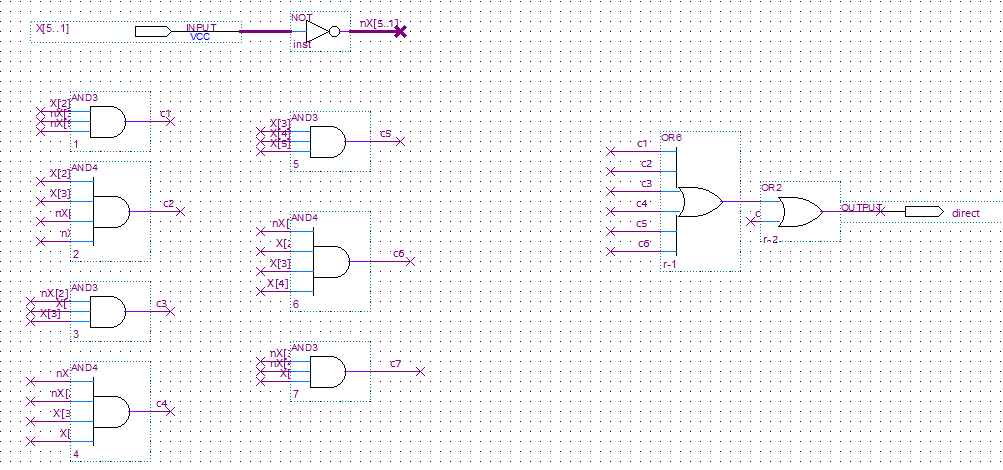
\includegraphics[width=\linewidth]{subfiles/images/scheme}
		\caption{Полученная схема}
		\label{fig:scheme}
	\end{figure}
	
	\begin{figure}[H]
		\centering
		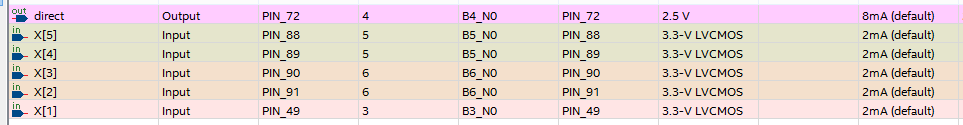
\includegraphics[width=\linewidth]{subfiles/images/pins}
		\caption{Назначенные сигналы}
		\label{fig:pins}
	\end{figure}
	
	\subsection{Анализ синтеза комбинационной схемы}
	Для начала воспользуемся RTL Viewer для рассмотрения преобразования
	логики в процессе синтеза. На рисунке видно, что существенных изменений
	не произошло, за исключением того, что теперь инверсия переменных
	реализуется на входах логических элементов.
	\begin{figure}[H]
		\centering
		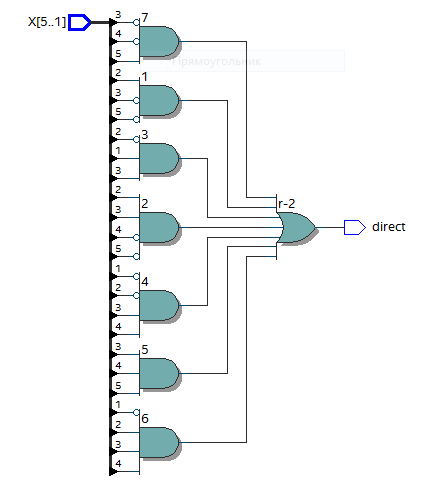
\includegraphics[width=0.5\linewidth]{subfiles/images/rtl}
		\caption{Логическое представление устройства в RTL Viewer}
		\label{fig:rtl}
	\end{figure}
	На основе полученного RTL описания в процессе синтеза в элементном
	базисе выбранной для проекта ПЛИС синтезируется новая схема (Netlist)
	с той же функциональностью, что и исходная схема. Синтезированное
	представление схемы в базисе целевой ПЛИС доступно в Technology Map Viewer.
	\begin{figure}[H]
		\centering
		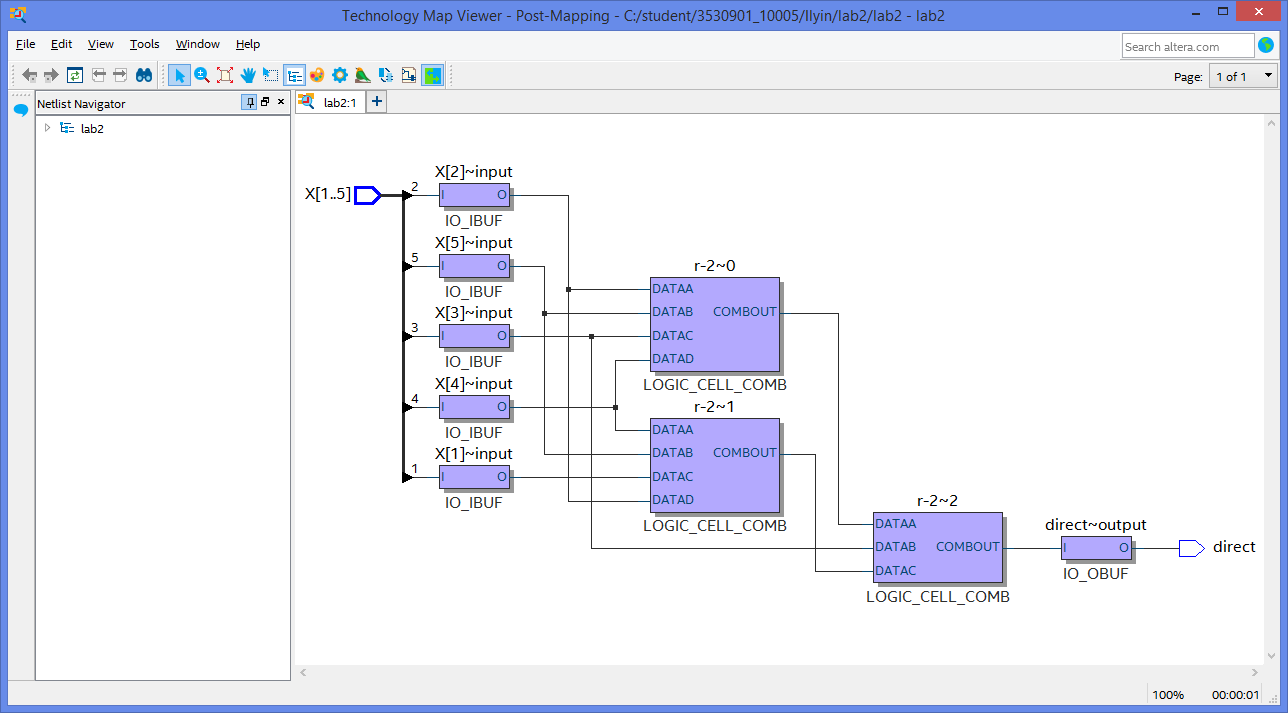
\includegraphics[width=\linewidth]{subfiles/images/tmv}
		\caption{Схема устройства в Technology Map Viewer}
		\label{fig:rmv}
	\end{figure}
	
	В редакторе временных диаграмм САПР QP создадим тест, в котором работа
	КС проверяется на всех наборах входных сигналов.
	\begin{figure}[H]
		\centering
		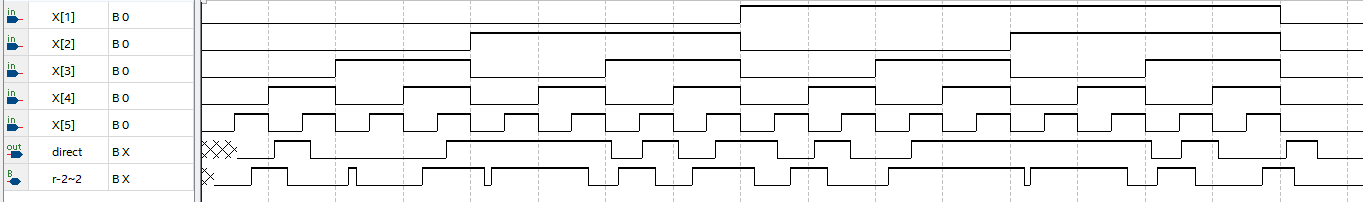
\includegraphics[width=\linewidth]{subfiles/images/wave}
		\caption{Временная диаграмма}
		\label{fig:wave}
	\end{figure}
	На диаграмме видно, что полученные выходные сигналы совпадают с ожидаемыми,
	следовательно, схема реализована верно. 
	
	Последним шагом в работе была реализация КС на физической модели.
	При помощи Quartus Prime, была запрограммирована микросхема
	miniDiLaB-CIV c ПЛИС Cyclone IV EP4CE6E22C8N, на которой при помощи переключателей и светодиодов 
	еще раз была проверена правильность работы логической функции.
	\begin{figure}[H]
		\centering
		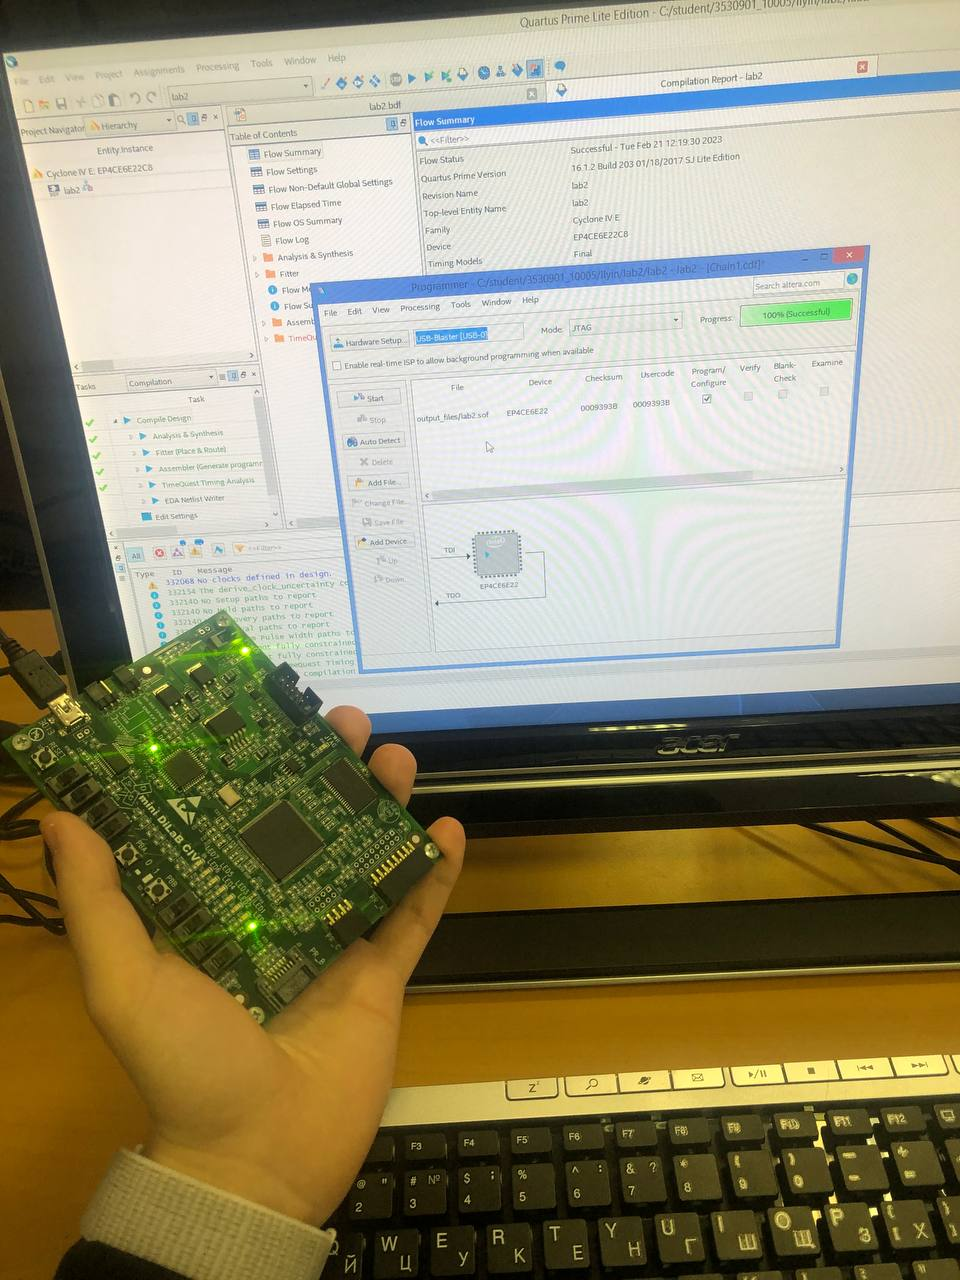
\includegraphics[width=0.5\linewidth]{subfiles/images/chip}
		\caption{Пример работы физической модели}
		\label{fig:chip}
	\end{figure}
	
	\section{Вывод}
	В результате работы заданная таблично логическая функция была минимизирована при помощи карт
	Карно. Была синтезирована и исследована комбинационная схема. В заключение, она была 
	реализована на физической модели.
\end{document}
